%% ---------------------------------------------------------------------------
%% 04_results.tex -- Results, Discussion, Conclusion
%% Figure floats carry the captions and the \label; the \includegraphics lines
%% are commented and are wired by the lead.
%% ---------------------------------------------------------------------------

\section{Results}
\label{sec:results}

All results below use one code version and one configuration file. Unless a
subsection says otherwise, the forcing is the chamber condition of the
reference experiment and the simulated period is 30 days. The shared
parameterisation has four fitted coefficients: $\lambda_{sb}$,
$\lambda_{sdr}$, $\lambda_{sdi}$ and the half-activation sucrose concentration
of the sink term. These values are the same at every photoperiod and are not
refitted between the studies below.

\subsection{Photoperiod-dependent relative growth rate}
\label{sec:results:rgr}

With the shared parameterisation the model gives a mean absolute percentage
error of $8.58\%$ in relative growth rate (RGR) across the four photoperiods,
and the worst photoperiod reaches $11.75\%$. All four scenarios integrate to
the end of the simulated period without a non-finite sample. Under the
acceptance criteria of Section~\ref{sec:protocol} the same parameterisation
gives a mean error of $8.88\%$, and 3 of the 4 photoperiods are accepted. The
4~h scenario is rejected on the RGR criterion alone. Table~\ref{tab:rgr} lists
the per-photoperiod values and Figure~\ref{fig:rgr} shows them against the
reference targets of \citet{Sulpice2014}.

The errors are not evenly distributed. The 4~h scenario is overestimated by
$15.04\%$, while the 6, 8 and 12~h scenarios stay between $4.77$ and $8.71\%$.
One parameter set therefore reproduces the magnitude and the direction of the
photoperiod response, but not its exact shape at the short end of the range.
Section~\ref{sec:results:envelope} shows that this residual has a structural
cause and not a calibration cause.

The growth response is large in absolute terms, which is worth stating because
RGR is a logarithmic rate and hides it. Final total biomass after 30 days rises
from $0.387$ gFW at 4~h to $1.258$ at 6~h, $4.006$ at 8~h and $39.03$ gFW at
12~h, a hundredfold spread produced by a threefold change in day length. The
errors quoted above are therefore errors in an exponent, and a $10\%$ error in
RGR compounds over the simulated period. Halving the output step changes the
simulated RGR and the final biomass by less than $0.01\%$ in all four
scenarios, so these differences come from the model and not from the
integration.

The saturated per-photoperiod regime behaves differently, and the contrast
matters. That regime fits two coefficients per photoperiod, eight against eight
observations, so it has zero degrees of freedom. Its per-photoperiod errors on
the grid used here are $3.42$, $1.28$, $2.45$ and $3.03\%$. These values are
set by the grid resolution of $2.5\times10^{-5}$ rather than by the model, and
refining the bisection drives them towards zero. They are convergence residuals
and carry no information about predictive skill. The point is not academic.
Evaluated under the chamber forcing used throughout this paper, the same
per-photoperiod parameterisation gives an RGR error of $48.67\%$, and none of
the four photoperiods is accepted. Near-zero residuals at the calibration point
with a large error one condition away are the expected signature of a saturated
fit.

\begin{table}[!htbp]
\centering
\caption{Relative growth rate under the shared parameterisation, chamber
forcing, 30 days. Targets are the \textit{Arabidopsis thaliana} rosette values
of \citet{Sulpice2014}. The last column gives the per-photoperiod residual of
the saturated per-photoperiod calibration on the grid described in
Section~\ref{sec:results:rgr}; those residuals are set by the grid resolution
and are reported as calibration diagnostics, not as errors of prediction.}
\label{tab:rgr}
\begin{tabular}{@{}lrrrcr@{}}
\toprule
Photoperiod & Target RGR & Simulated RGR & Error & Accepted & Saturated fit \\
(h) & (d$^{-1}$) & (d$^{-1}$) & (\%) & & residual (\%) \\
\midrule
4  & 0.0680 & 0.0782 & 15.04 & no  & 3.42 \\
6  & 0.1135 & 0.1189 &  4.77 & yes & 1.28 \\
8  & 0.1708 & 0.1588 &  7.00 & yes & 2.45 \\
12 & 0.2600 & 0.2374 &  8.71 & yes & 3.03 \\
\midrule
\multicolumn{3}{@{}l}{Mean absolute percentage error} & 8.88 & 3/4 & -- \\
\bottomrule
\end{tabular}
\end{table}

\begin{figure}[!htbp]
\centering
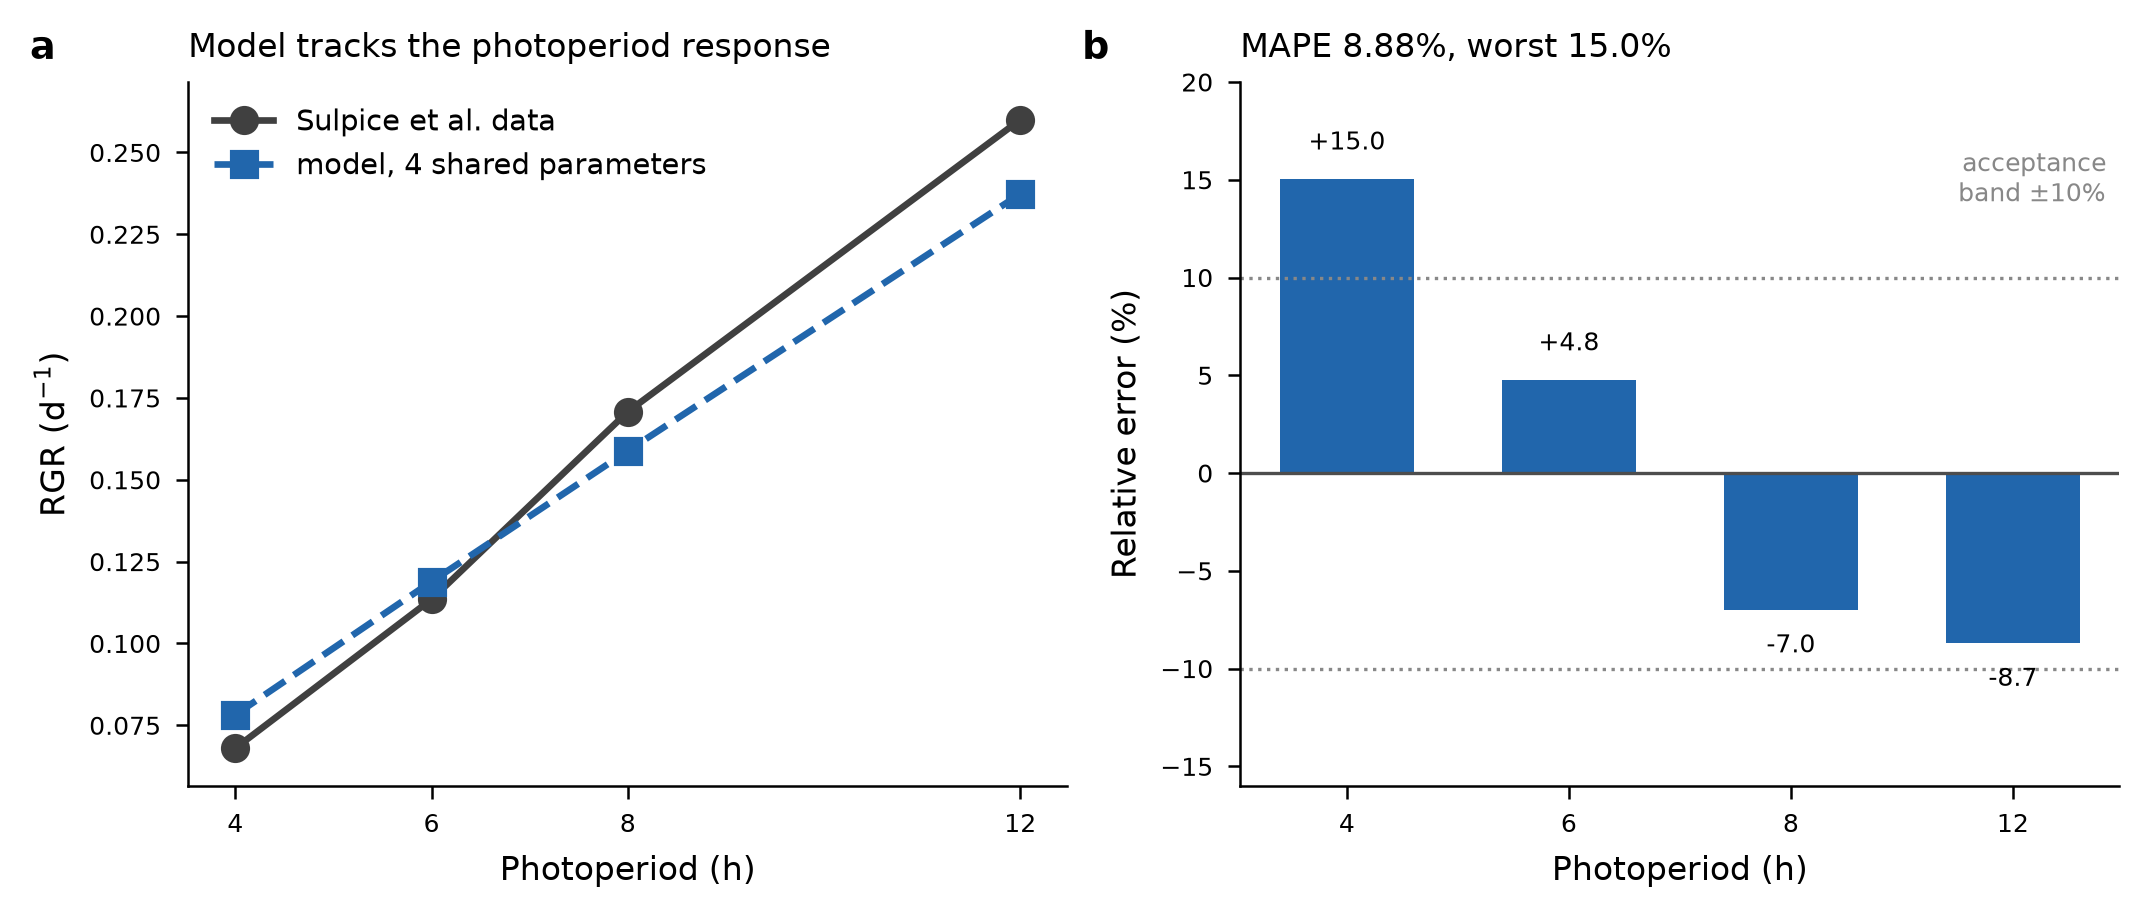
\includegraphics[width=\linewidth]{rgr_validation.png}
\caption{Relative growth rate against photoperiod. Simulated values under the
shared four-parameter parameterisation are compared with the reference targets
of \citet{Sulpice2014} for 4, 6, 8 and 12~h photoperiods. The residuals of the
saturated per-photoperiod calibration are shown for reference only; they are
convergence residuals of a fit with zero degrees of freedom.}
\label{fig:rgr}
\end{figure}

\subsection{Cross-photoperiod prediction}
\label{sec:results:crossval}

The held-out test asks a different question: how well does the model predict a
photoperiod that was not used to fit anything? We fitted the growth coefficient
on three photoperiods, predicted the fourth, and repeated this for each of the
four folds. Table~\ref{tab:crossval} reports both regimes and
Figure~\ref{fig:crossval} shows the predictions.

In regime A the growth coefficient is one shared constant. The held-out error is
$13.18\%$ and the worst fold is $20.93\%$, with the 4~h treatment held out. In
regime B the same coefficient depends linearly on photoperiod $P$,

\begin{equation}
\lambda_{sb}(P) = c_0 + c_1 P,
\label{eq:lsb_linear}
\end{equation}

with two coefficients instead of one. The held-out error falls to $4.36\%$ and
the worst fold is $10.30\%$, now at the 12~h treatment. The fitted values are
$c_0 = 0.00243$ and $c_1 = 8.786\times10^{-5}$ per hour. Across the four folds
the fitted growth coefficient rises monotonically with photoperiod, from
$0.00275$ at 4~h to $0.00370$ at 12~h. Adding one coefficient therefore
predicts an unseen photoperiod about three times better than a single
constant.

Two readings follow. First, the growth coefficient is not photoperiod-invariant
in this model. If the coupled dynamics generated the full photoperiod response,
a shared constant would be enough and regime B would add nothing. Second, the
missing dependence is compact. A straight line in one coefficient captures it
over the tested range, which places it in the conversion from available sucrose
to structural growth rather than in the gas-exchange layer upstream. A positive
slope means that a longer day converts loaded sucrose into biomass more
efficiently, not only for longer. Increased sink activity under long days is a
plausible reading \citep{Smith2007,Sulpice2014}, but the design cannot separate
it from an allocation effect or from a fresh-weight conversion effect.

The limits of Eq.~\ref{eq:lsb_linear} belong with the result. The line was
fitted over 4 to 12~h and has no support outside that interval. It corrects a
model coefficient and does not describe a process, so extrapolating it to 18 or
24~h has no basis. It must also break down at short photoperiods, because the
coefficient would reach zero at a positive day length.

\begin{table}[!htbp]
\centering
\caption{Leave-one-photoperiod-out prediction of relative growth rate. In
regime A the growth coefficient is a single shared constant; in regime B it is
linear in photoperiod with two coefficients (Eq.~\ref{eq:lsb_linear}). Train
error is the mean over the three fitted photoperiods; test error is the
held-out photoperiod. The $\lambda_{sb}$ column gives the value applied at the
held-out photoperiod.}
\label{tab:crossval}
\begin{tabular}{@{}llrrr@{}}
\toprule
Regime & Held out (h) & $\lambda_{sb}$ & Train MAPE (\%) & Test MAPE (\%) \\
\midrule
A: shared constant & 4  & 0.00320 & 5.57 & 20.93 \\
A: shared constant & 6  & 0.00320 & 9.24 &  9.94 \\
A: shared constant & 8  & 0.00295 & 8.08 & 10.10 \\
A: shared constant & 12 & 0.00295 & 7.53 & 11.75 \\
\midrule
\multicolumn{4}{@{}l}{Regime A, mean held-out error} & 13.18 \\
\midrule
B: linear in $P$ & 4  & 0.00275 & 2.25 &  3.42 \\
B: linear in $P$ & 6  & 0.00295 & 2.97 &  1.28 \\
B: linear in $P$ & 8  & 0.00320 & 2.57 &  2.45 \\
B: linear in $P$ & 12 & 0.00370 & 2.38 & 10.30 \\
\midrule
\multicolumn{4}{@{}l}{Regime B, mean held-out error} & 4.36 \\
\bottomrule
\end{tabular}
\end{table}

\begin{figure}[!htbp]
\centering
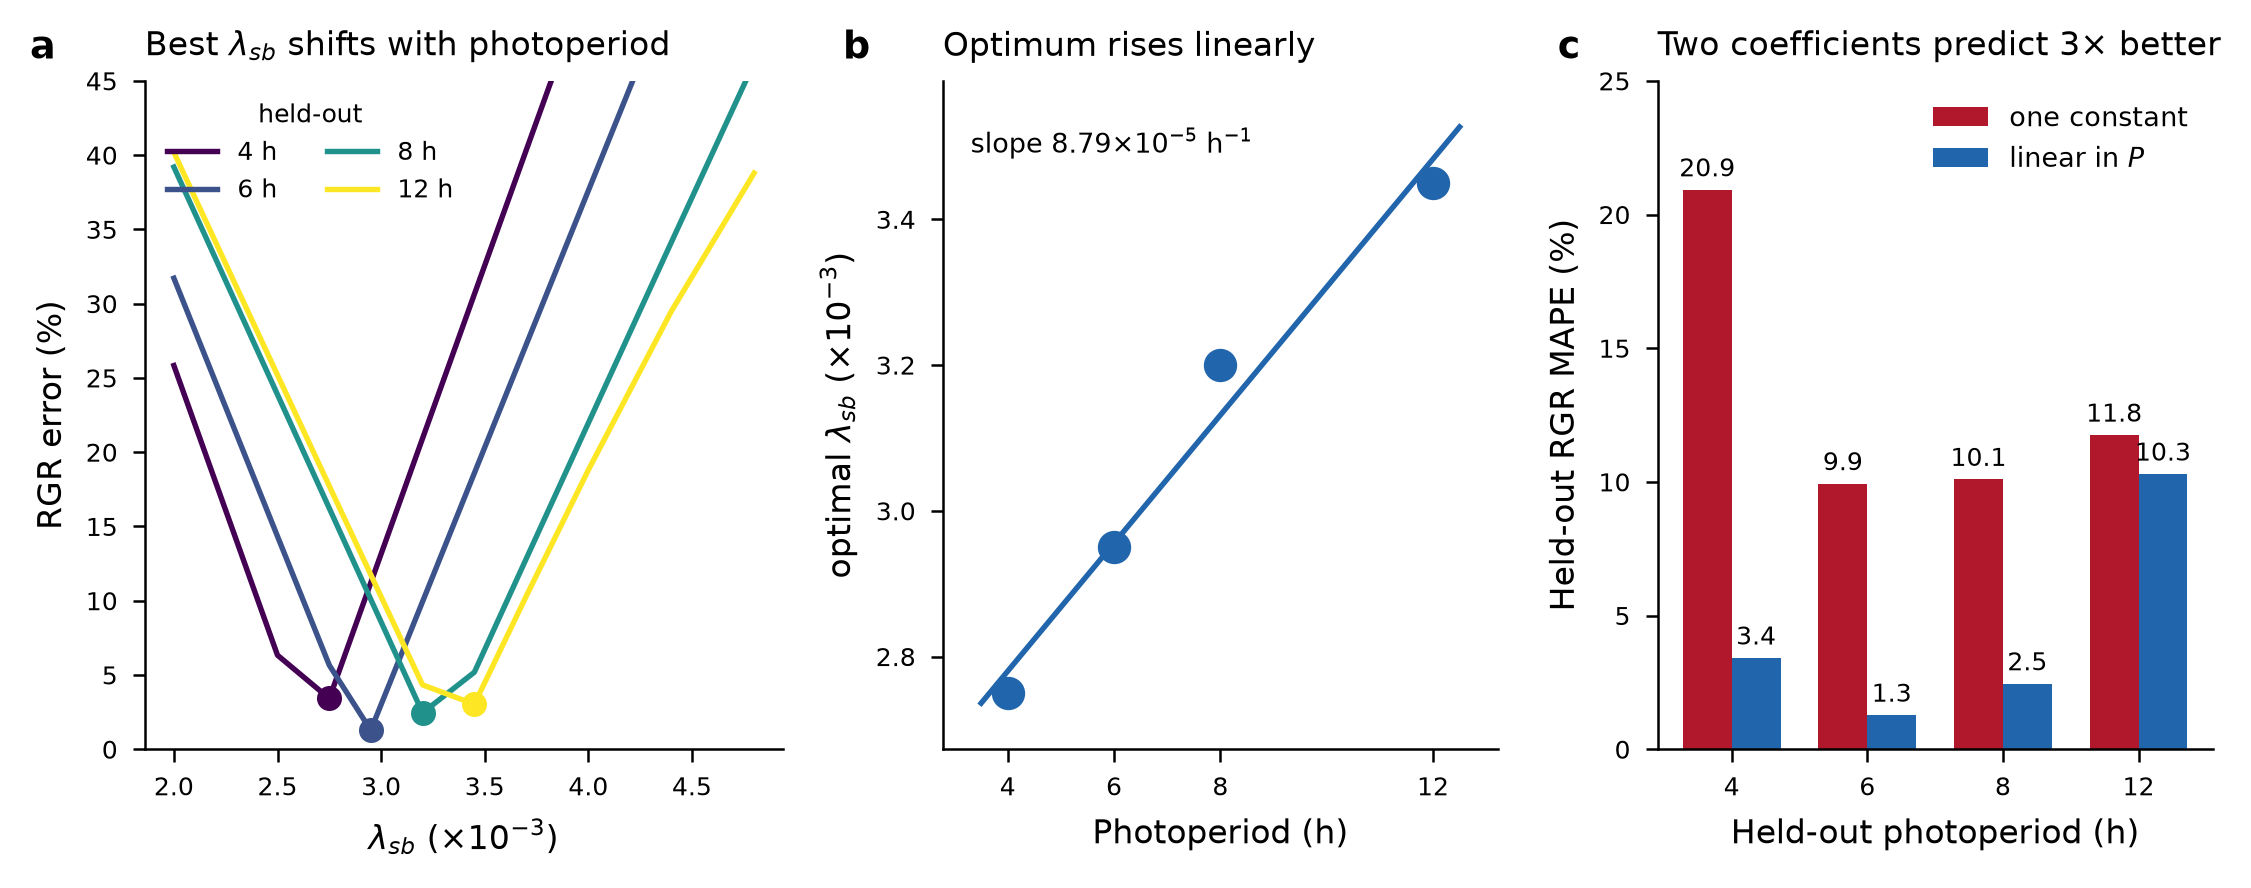
\includegraphics[width=\linewidth]{crossval.png}
\caption{Held-out photoperiod prediction of relative growth rate. Regime A
uses one shared growth coefficient; regime B lets the same coefficient vary
linearly with photoperiod (Eq.~\ref{eq:lsb_linear}). Each point is a
photoperiod that was excluded from the fit that produced it.}
\label{fig:crossval}
\end{figure}

\subsection{Diel carbohydrate dynamics}
\label{sec:results:carb}

The carbohydrate comparison uses one multiplicative scale per series, fitted
by least squares before the error is computed, so the normalised RMSE scores
the shape and the timing of the diel cycle. Over the reference series the mean
starch nRMSE is $0.235$ against the acceptance threshold of $0.25$, with a bias
of $-3.1\%$. The mean sucrose nRMSE is $0.285$ against a threshold of $0.50$,
with a bias of $+10.7\%$. In the validation runs the largest per-photoperiod
values are $0.219$ for starch and $0.468$ for sucrose. Figure~\ref{fig:carb}
shows the traces.

The two series are not equally strong, and the fitted scales show why. For
starch the scale is between $0.86$ and $1.15$ over the four fitted
photoperiods, so shape and absolute level both agree and the starch nRMSE
means what a reader would assume it means. For sucrose the scale is between
$2.25$ and $3.31$: the simulated pool must be multiplied by a factor of two to
three before it matches the measurements. Raw simulated sucrose maxima are
$1.30$ to $1.40~\mu\mathrm{mol}$ C$_6$ gFW$^{-1}$ against measured maxima of
$3.18$ to $4.71~\mu\mathrm{mol}$ C$_6$ gFW$^{-1}$. The passing sucrose nRMSE
of $0.285$ therefore describes shape and timing only, and the absolute sucrose
level is a known deficit of this version. We report the scale factor beside
every carbohydrate error for that reason.

Within the fitted range the model reproduces the qualitative features of the
diel cycle. Starch accumulates through the light period and degrades through the
night along a near-linear trajectory. At dawn it returns to the level at which
each run started, so the pool is close to empty at the end of every night. This
behaviour follows from the drain law of
Section~\ref{sec:carbohydrates}, which targets the remaining pool over the
remaining night, and it agrees with the near-linear nocturnal degradation
reported for \textit{Arabidopsis} \citep{Graf2010,Scialdone2013}.

One quantitative feature is not reproduced. The measured end-of-day starch
peak grows more steeply with photoperiod than the simulated peak. In the model
the peak does rise with photoperiod, because the light period is longer, but the
rise is weaker than measured. The model therefore under-represents how much a
long day changes the size of the transient store, as opposed to its filling
time. The same shortfall appears from the other side in
Section~\ref{sec:results:envelope}, where assimilation per light hour is found
to be constant.

\begin{figure}[!htbp]
\centering
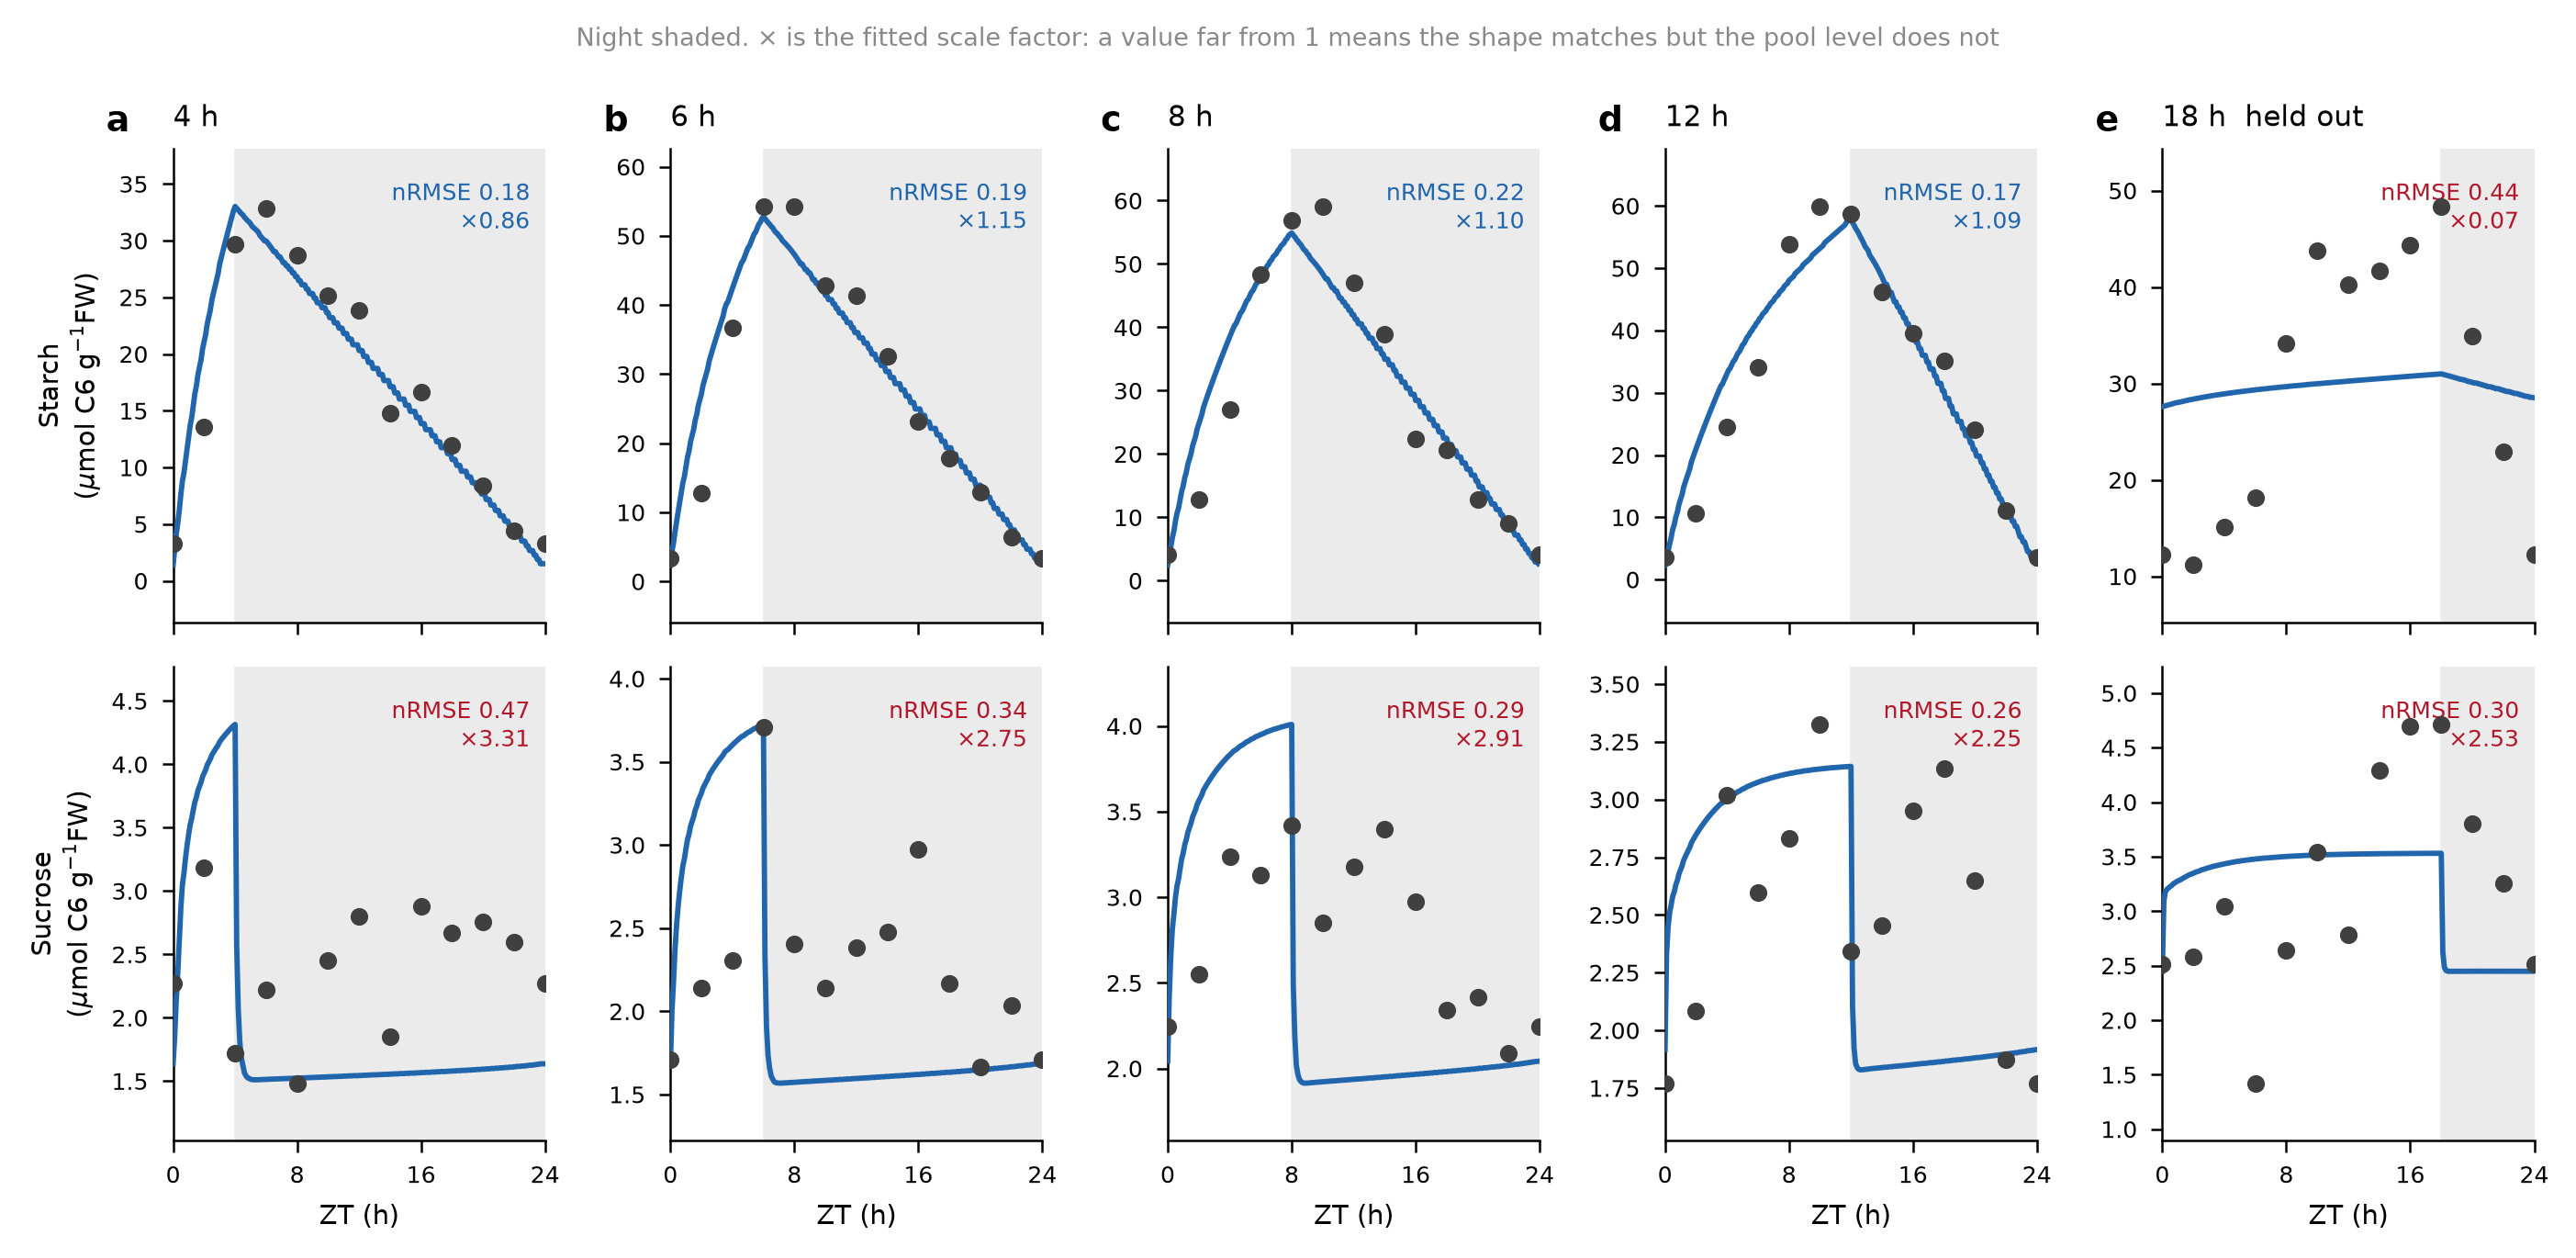
\includegraphics[width=\textwidth]{carbohydrate_diel.png}
\caption{Diel starch and sucrose dynamics for the 4, 6, 8, 12 and 18~h
photoperiods. Simulated traces are compared with the measured diel profiles of
the repository reference file (see Section~\ref{sec:protocol}). Each panel prints the nRMSE and
the fitted multiplicative scale. The scale is between $0.86$ and $1.15$ for
starch at the four fitted photoperiods and between $2.25$ and $3.31$ for
sucrose, so the sucrose comparison is one of shape and timing and not of
absolute level. The 18~h column was not used in any fit; its starch nRMSE is
not reported, because the fitted scale of $0.07$ absorbs the divergence
described in Section~\ref{sec:results:envelope}.}
\label{fig:carb}
\end{figure}

\subsection{Ablation}
\label{sec:results:ablation}

The ablation compares three carbon-input pathways with the same downstream
model, the same shared parameters and no refitting. In M0 the carbon input is
prescribed. In M1 it is computed from Farquhar photosynthesis
\citep{Farquhar1980} at fixed stomatal conductance. In M2 the conductance
follows the Jarvis formulation \citep{Jarvis1976} and responds to the
environment. Table~\ref{tab:ablation} and Figure~\ref{fig:ablation} give the
result: the RGR error falls from $41.01\%$ for M0 to $9.43\%$ for M1 and to
$8.88\%$ for M2.

The large step is from prescribed to computed carbon input. M0 underestimates
RGR at every photoperiod, by $39.2$ to $43.1\%$, and its peak assimilation
stays between $10.50$ and $11.14~\mu\mathrm{mol}$ gFW$^{-1}$ h$^{-1}$. With
computed assimilation the peak rises to $17.62$ and the systematic
underestimation disappears. The bias is not reduced but removed: M1 and M2
scatter on both sides of the targets, while M0 is low in all four scenarios.
Parameters were frozen across the three variants, so the change comes from the
carbon-input pathway and not from recalibration.

The Jarvis layer adds a smaller and unevenly distributed gain. Averaged over
the four photoperiods it reduces the error from $9.43$ to $8.88\%$, and the two
variants differ most at the extremes of the range. At 4~h, M2 improves on M1
by $3.8$ percentage points, from $18.82$ to $15.04\%$. At 12~h it is worse by
$2.1$ points, $8.71$ against $6.60\%$. At 6~h M2 is better by $3.0$ points and
at 8~h it is worse by $2.5$ points. Adding environmental control of conductance lowers peak
assimilation slightly, from $17.62$ to $17.01~\mu\mathrm{mol}$ gFW$^{-1}$
h$^{-1}$, because the conductance multipliers are below one at the nominal
condition. The value of M2 at a single nominal condition is therefore not a
gain in RGR accuracy. Its value is that the carbon input responds to
irradiance, humidity, temperature, ambient CO$_2$ and leaf water potential at
all, which is what the sensitivity analysis of the next subsection exercises.

\begin{table}[!htbp]
\centering
\caption{Ablation of the carbon-input pathway. M0 prescribes the carbon input,
M1 computes it from Farquhar photosynthesis at fixed conductance, and M2 adds
Jarvis stomatal conductance. Shared parameters are frozen across the three
variants. Errors are relative errors in RGR; the last column is the peak
assimilation rate.}
\label{tab:ablation}
\begin{tabular}{@{}lrrrrrr@{}}
\toprule
& \multicolumn{4}{c}{RGR error (\%) by photoperiod} & MAPE & Peak $\Phi_c$ \\
Variant & 4~h & 6~h & 8~h & 12~h & (\%) & ($\mu$mol gFW$^{-1}$h$^{-1}$) \\
\midrule
M0 prescribed        & 41.59 & 40.19 & 43.08 & 39.20 & 41.01 & 10.50--11.14 \\
M1 Farquhar          & 18.82 &  7.77 &  4.55 &  6.60 &  9.43 & 17.62 \\
M2 Farquhar--Jarvis  & 15.04 &  4.77 &  7.00 &  8.71 &  8.88 & 17.01 \\
\bottomrule
\end{tabular}
\end{table}

\begin{figure}[!htbp]
\centering
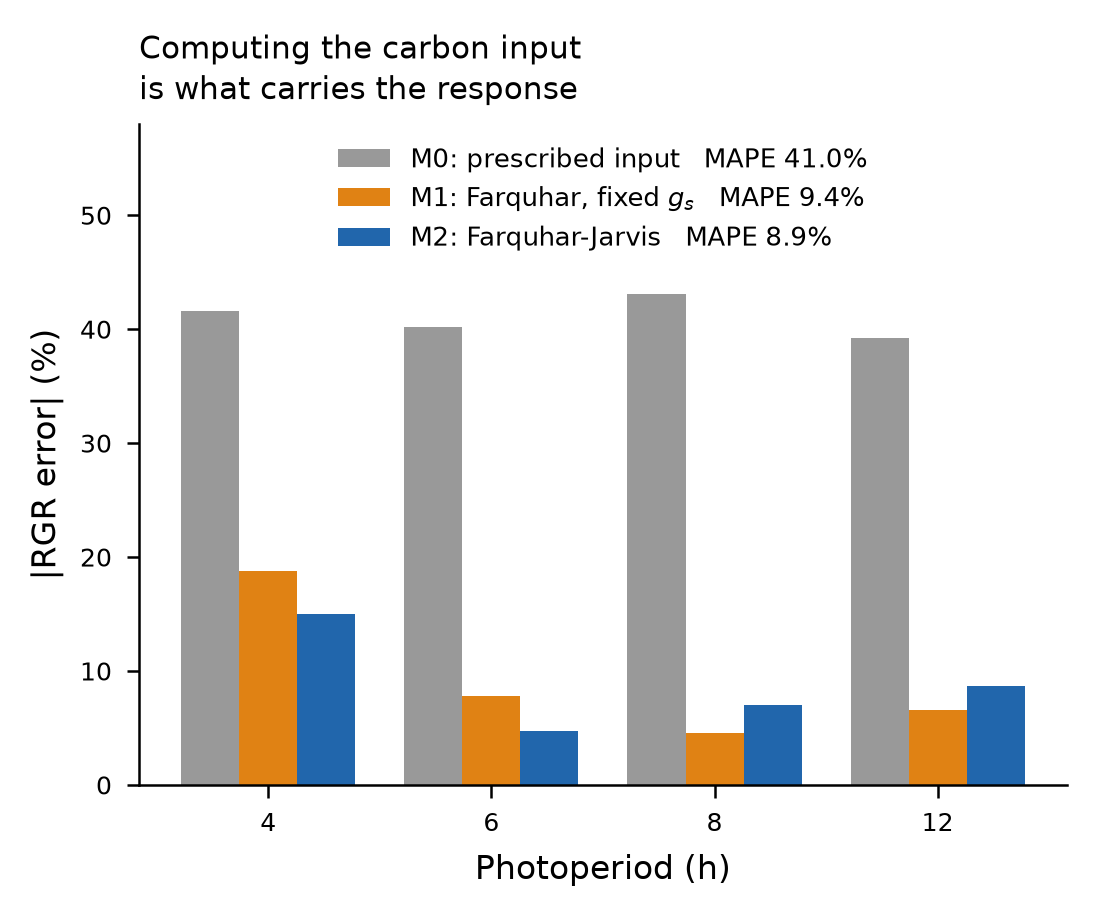
\includegraphics[width=0.58\linewidth]{ablation.png}
\caption{Relative RGR error per photoperiod for the three carbon-input
variants, with shared parameters frozen. M0 underestimates growth at every
photoperiod; M1 and M2 scatter on both sides of the targets.}
\label{fig:ablation}
\end{figure}

\subsection{Global sensitivity}
\label{sec:results:sens}

The variance-based analysis follows \citet{Sobol2001} with the estimator of
\citet{Saltelli2010}, and the Morris screening follows
\citet{Morris1991,Campolongo2007}. Sixteen parameters were varied over the
declared ranges of Appendix~\ref{app:sa}. Table~\ref{tab:sens} gives the full
ranking and Figure~\ref{fig:sens} shows the total-order indices next to the
Morris measures.

Nutrient uptake capacity dominates the total-order ranking. The two largest
total indices are $0.658$ for maximum phosphorus uptake and $0.577$ for maximum
nitrogen uptake. Respiration frequency follows at $0.466$, then ambient CO$_2$
concentration at $0.422$ and leaf water potential at $0.412$. The two Farquhar
capacities come next, $0.352$ for electron transport rate and $0.334$ for
maximum carboxylation rate, then maximum PAR at $0.333$. The ranking spans the
nutrient, respiratory and gas-exchange blocks, as expected in a model where
growth is limited by whichever supply is scarcest.

The main-effect share is small. Summed over the sixteen parameters and averaged
over the four photoperiods, the first-order indices give $0.201$ against a
summed total-order index of $4.675$, a main-effect share of about $4\%$. The
Morris measures agree: 15 of the 16 parameters have $\sigma/\mu^{*} > 1$, and
the exception is the one parameter with a total index at noise level. The two
methods also rank the parameters consistently, with a Spearman rank correlation
of $\rho = 0.944$ between Morris $\mu^{*}$ and Sobol' $S_T$. The model is
interaction-dominated over the declared ranges: parameters act mainly through
each other, not on their own.

A low main-effect share can also be an estimator artefact, so we checked
convergence with sample size. As $n$ rises from $512$ to $4096$, the number of
first-order estimates clipped at zero falls from $8$ to $3$. Over the same
range the summed first-order index stays between $0.151$ and $0.340$, and the
main-effect share stays between $3.0$ and $6.4\%$. The clipping decreases, which is what an
estimator with shrinking variance should do, but the share does not increase
with it. The low main-effect share is therefore a property of the model over
these ranges and not an artefact of a small sample. All indices in
Table~\ref{tab:sens} are reported unclipped, so small negative interaction
remainders appear where an index is at noise level; we prefer that to hiding
the estimator variance.

One entry deserves a comment. The growth coefficient $\lambda_{sb}$, the
coefficient that Section~\ref{sec:results:crossval} shows to carry the
photoperiod response, has a total index of only $0.117$ and ranks fifteenth of
sixteen. There is no contradiction. A Sobol' index measures the variance
contribution over a declared range at fixed forcing, while the
cross-photoperiod result measures how a coefficient must change when the
forcing changes. A parameter can be unimportant for variance at one condition
and still be the parameter that fails to transfer between conditions.

\begin{table}[!htbp]
\centering
\caption{Global sensitivity of relative growth rate, averaged over the four
photoperiods. $S_1$ is the first-order and $S_T$ the total-order Sobol' index;
the interaction remainder is $S_T - S_1$. $\mu^{*}$ and $\sigma$ are the
Morris measures. Indices are reported unclipped, so a remainder at noise level
can be slightly negative. Ranges and sampling scales are in
Appendix~\ref{app:sa}; the indices are conditional on those ranges.}
\label{tab:sens}
\footnotesize
\begin{tabular}{@{}lrrrrr@{}}
\toprule
Parameter & $S_1$ & $S_T$ & $S_T-S_1$ & $\mu^{*}$ & $\sigma/\mu^{*}$ \\
\midrule
\texttt{max\_phosphorus\_uptake}   & 0.000 & 0.658 & 0.658 & 0.635 & 1.73 \\
\texttt{max\_nitrogen\_uptake}     & 0.000 & 0.577 & 0.577 & 0.785 & 1.48 \\
\texttt{respiration\_frequency}    & 0.031 & 0.466 & 0.435 & 0.466 & 1.94 \\
\texttt{ambient\_CO2\_concentration} & 0.000 & 0.422 & 0.422 & 0.370 & 2.13 \\
\texttt{leaf\_water\_potential}    & 0.063 & 0.412 & 0.349 & 0.597 & 1.57 \\
\texttt{electron\_transport\_rate} & 0.020 & 0.352 & 0.332 & 0.247 & 2.57 \\
\texttt{max\_rubisco\_carboxylation\_rate} & 0.013 & 0.334 & 0.321 & 0.393 & 2.16 \\
\texttt{max\_PAR}                  & 0.000 & 0.333 & 0.333 & 0.463 & 1.96 \\
\texttt{leaf\_temperature}         & 0.008 & 0.219 & 0.211 & 0.198 & 3.05 \\
\texttt{relative\_humidity}        & 0.000 & 0.199 & 0.199 & 0.222 & 2.84 \\
\texttt{phosphorus\_soil\_content} & 0.017 & 0.164 & 0.148 & 0.202 & 2.62 \\
\texttt{sucrose} (initial)         & 0.007 & 0.144 & 0.137 & 0.164 & 2.70 \\
\texttt{nitrogen\_soil\_content}   & 0.007 & 0.141 & 0.134 & 0.100 & 3.72 \\
\texttt{k\_vacuole\_in}            & 0.009 & 0.135 & 0.126 & 0.101 & 3.96 \\
\texttt{lambda\_sb}                & 0.023 & 0.117 & 0.094 & 0.073 & 3.32 \\
\texttt{total\_biomass} (initial)  & 0.003 & 0.001 & $-0.002$ & 0.066 & 0.37 \\
\midrule
Sum & 0.201 & 4.675 & & & \\
\bottomrule
\end{tabular}
\end{table}

\begin{figure}[!htbp]
\centering
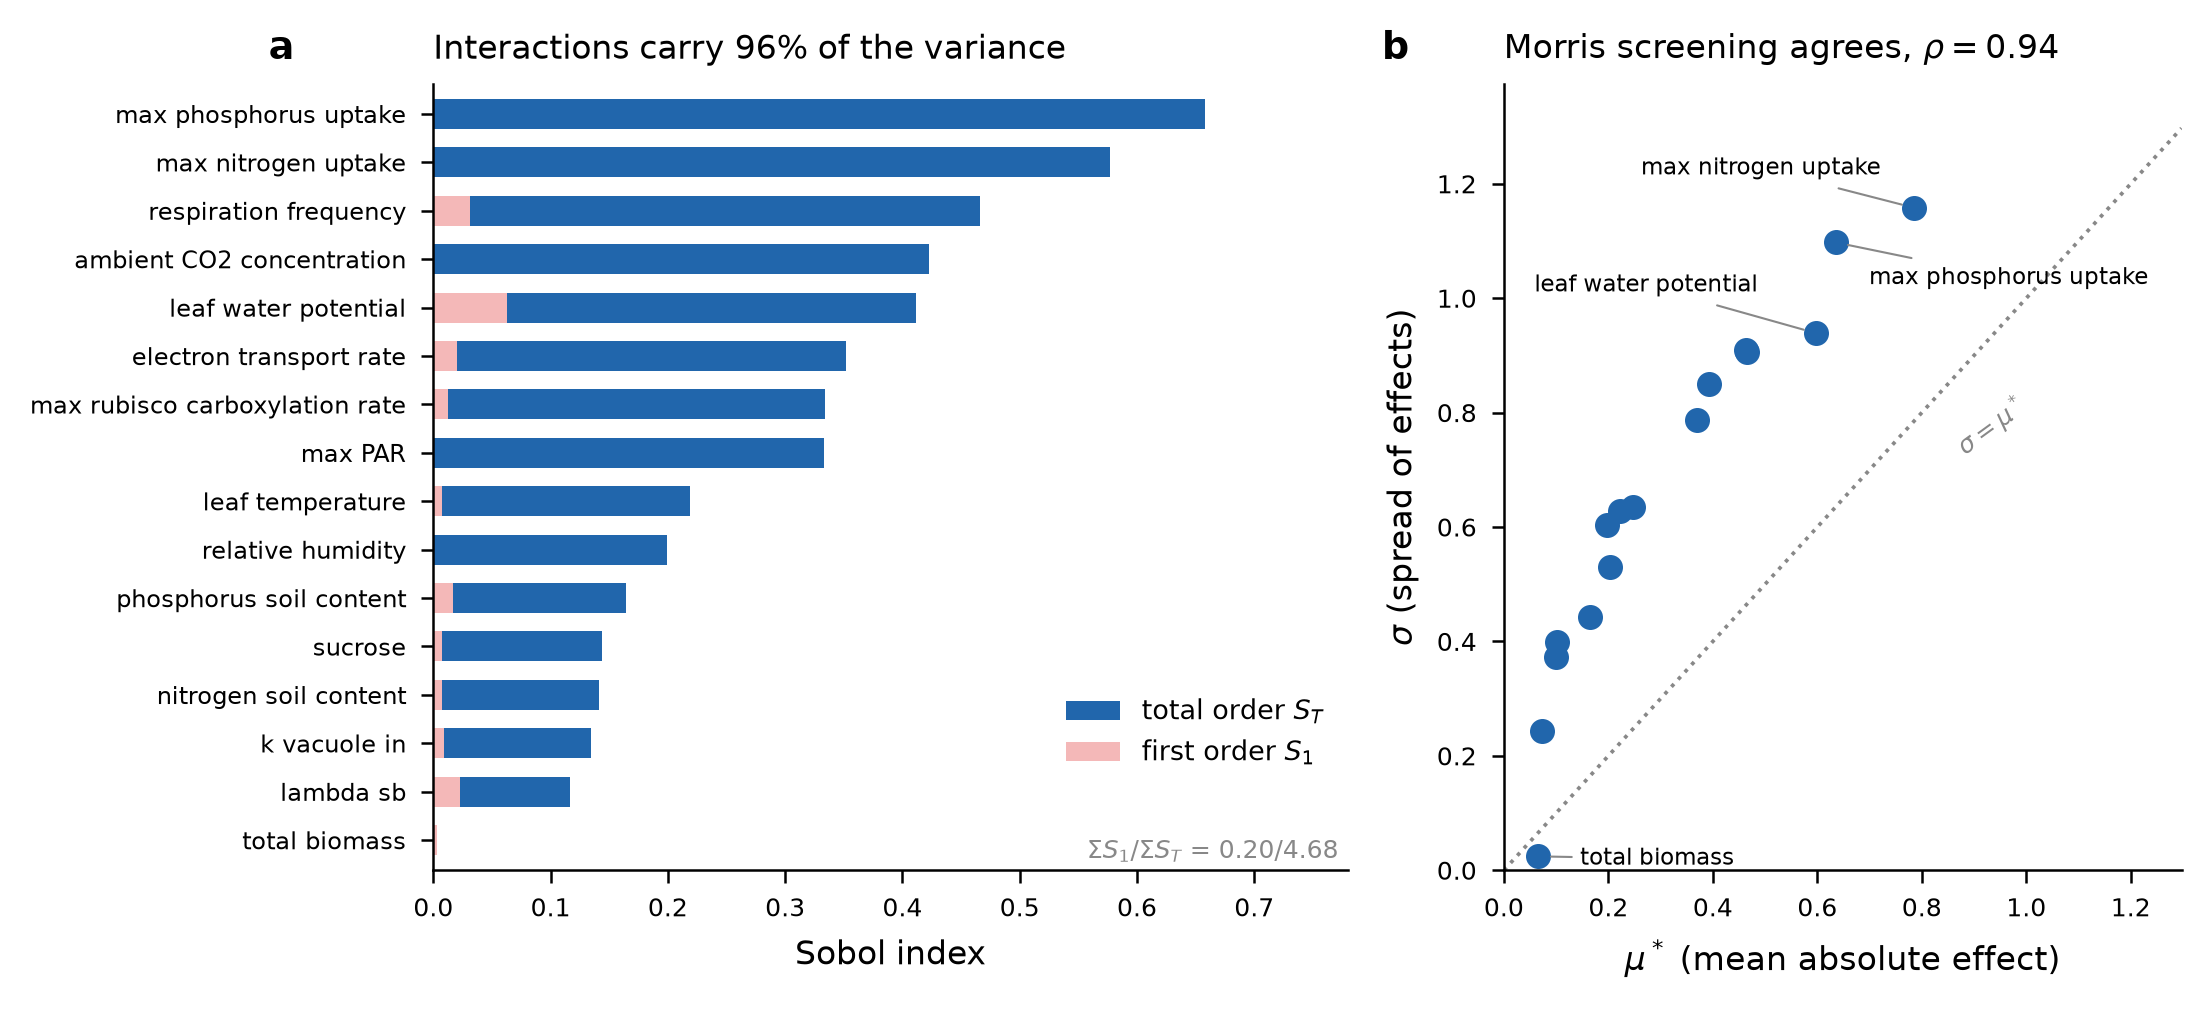
\includegraphics[width=\textwidth]{sensitivity.png}
\caption{Global sensitivity of relative growth rate over the declared
parameter ranges. Left: total-order Sobol' indices with the first-order part
shown separately. Right: Morris $\mu^{*}$ and $\sigma$. The two rankings agree
at a Spearman correlation of $0.944$, and 15 of the 16 parameters have
$\sigma/\mu^{*} > 1$.}
\label{fig:sens}
\end{figure}

\subsection{Validity envelope}
\label{sec:results:envelope}

Two limits of the model were measured directly, and we report them as findings
rather than as caveats. Figure~\ref{fig:envelope} shows both.

The first limit is the 18~h photoperiod, which was never used in any fit. The
sucrose comparison passes: nRMSE is $0.428$ against the threshold of $0.50$,
with a fitted scale of $2.53$, so the shape of the diel sucrose cycle survives
three hours beyond the fitted range. The starch pool does not. Dawn starch is
$401~\mu\mathrm{mol}$ gFW$^{-1}$ on day 30 and $1207~\mu\mathrm{mol}$ gFW$^{-1}$
on day 90, a net gain of about $+14$ per day that shows no sign of levelling
off. This is unbounded accumulation and not a wrong steady level, and the
distinction matters, because a wrong level can be rescaled while a divergence
cannot. The fitted scale for 18~h starch is $0.07$, which is the metric
absorbing the divergence, so no 18~h starch nRMSE is quoted anywhere in this
paper.

The mechanism is visible in the fluxes. The degradation cap is not binding at
18~h, so the failure is not a saturated drain. The drain law targets the
remaining pool over the remaining night, so nightly export is proportional to
what is left and to the reciprocal of the night length. Under a long day the
pool filled during the light period grows while the night available to empty it
shrinks. The day fill then outruns the drain, the pool carries a surplus into
the next day, and the surplus compounds.

The second limit is the closure boundary. Under the chamber forcing the net
daily starch gain is $+0.300$ at 12~h, $+0.295$ at 14~h and $+0.389$ at
15.0~h, rising to $+0.547$ at 15.5~h, $+2.042$ at 16~h, $+13.780$ at 18~h and
$+24.150$ at 20~h. The diel balance therefore closes up to $15.0$--$15.5$~h and
fails from 16~h. That boundary sits three hours beyond the longest photoperiod
used in any fit, which is a real margin and a narrow one.

The boundary is a property of the model and of the light dose together, not of
the model alone. Under the shipped half-sine profile at
$1200~\mu\mathrm{mol}$ m$^{-2}$ s$^{-1}$ the same measurement gives $+18.99$
at 12~h, $+32.56$ at 14~h, $+38.75$ at 15~h, $+45.00$ at 16~h, $+56.70$ at
18~h and $+67.68$ at 20~h. Under that dose the balance never closes, not even
at 12~h. Any statement of the form ``the model closes the diel starch balance
up to $P$ hours'' is therefore incomplete without the irradiance at which it
was measured. We report the chamber column as the envelope of this model, because it is the
condition with an experimental counterpart. The shipped column shows how
strongly the boundary depends on the daily photon dose.

The third measurement is a bound rather than a boundary, and it explains the
residual error of Section~\ref{sec:results:rgr}. Assimilation per hour of light
is constant to six significant figures across the photoperiod series, so total
daily assimilation is proportional to day length. The ratio of daily
assimilation between the 12 and 4~h scenarios is therefore exactly
$3.0000$, while the reference RGR targets require a ratio of $3.82$. Growth in
this model is driven by the carbon input, so a supra-proportional factor of
$1.27$ has to come from somewhere else. Partitioning cannot supply it: the
partition coefficients redistribute a fixed daily input between starch,
sucrose and biomass, and they cannot make the total larger. This is the same
gap that Eq.~\ref{eq:lsb_linear} closes empirically, seen at the level of the
carbon budget instead of the fitted coefficient.

\begin{figure}[!htbp]
\centering
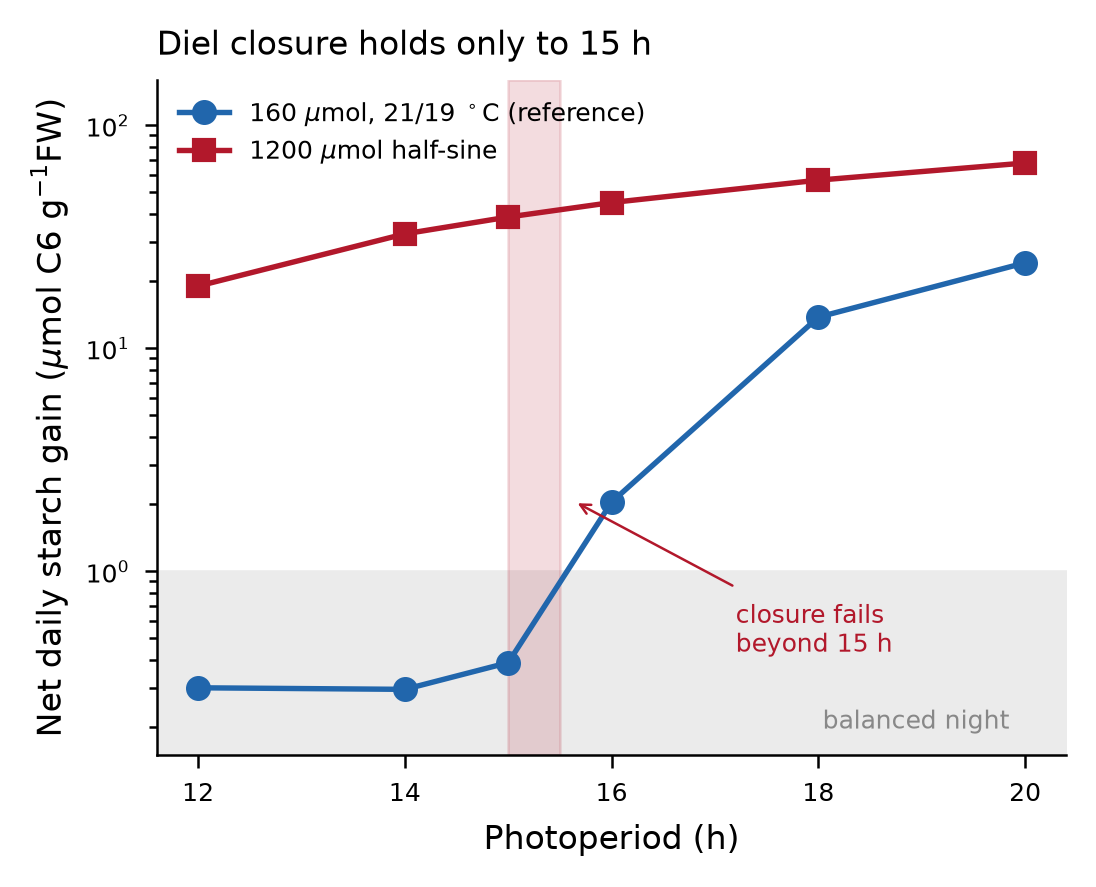
\includegraphics[width=0.58\linewidth]{validity_envelope.png}
\caption{Net daily starch gain against photoperiod on a symmetric-log axis,
under the chamber forcing and under the shipped half-sine profile at
$1200~\mu\mathrm{mol}$ m$^{-2}$ s$^{-1}$. The band marks the closure boundary
at $15.0$--$15.5$~h under chamber forcing. Under the higher dose the balance
does not close at any photoperiod shown, so the boundary depends on the light
dose as well as on the model.}
\label{fig:envelope}
\end{figure}

\section{Discussion}
\label{sec:discussion}

\subsection{What the coupled formulation buys}

The ablation puts a number on the coupling. Replacing a prescribed carbon input
with a computed one reduces the RGR error from $41.01$ to $9.43\%$ with no
parameter refitted. It removes a bias rather than reducing a scatter: M0 is low
at all four photoperiods, M1 and M2 are not. The reason is visible in the
assimilation rate. A prescribed maximum rate has to be chosen once, and a single
choice cannot be correct at four day lengths. The plant it describes has a
different leaf area and a different sucrose status in each case. The
computed input is a function of the states and of the forcing, so it changes
with them.

The Jarvis layer should be read differently. It reduces the mean error from
$9.43$ to $8.88\%$, which is a small change, and it moves the error in opposite
directions at the two ends of the photoperiod range. Reporting that as an
accuracy gain would misstate it. What the layer provides is a carbon input that
responds to irradiance, humidity, temperature, ambient CO$_2$ and leaf water
potential. The sensitivity analysis shows this is not a formality: ambient
CO$_2$ has a total-order index of $0.422$, leaf water potential $0.412$ and
maximum PAR $0.333$. In M1 those three parameters would move nothing through
the conductance path. A model intended for use across environments needs that
path even when it does not improve a single nominal-condition metric, and a
model evaluated only at its calibration point cannot show the difference.

This is where the model sits relative to existing families. It is not a
field-scale crop simulator, and it does not resolve architecture as a
functional-structural model does. It is a compact whole-plant core in which the
carbon input is computed from the environment and then propagated explicitly
into carbohydrate, nutrient and biomass states, with the numerical treatment and
the evaluation protocol stated. Many whole-plant and crop simulators prescribe
that input \citep{Holzworth2014,Jones2003,deWit2019}, and the ablation measures
what prescribing it costs in this setting. The physiological submodels are
inherited \citep{Farquhar1980,Jarvis1976,vonCaemmerer2000}; the coupling, the
analytic closure and the evaluation are what this paper contributes.

\subsection{Parameter transferability and what the design exposed}

The cross-photoperiod result is the part of this work with the widest reach
beyond plant modelling. One shared growth coefficient predicts a held-out
photoperiod with $13.18\%$ error; the same coefficient made linear in
photoperiod predicts it with $4.36\%$. Both regimes use the same equations, the
same states and the same solver. The difference is entirely in how one
coefficient is allowed to depend on a condition of the experiment.

That is a statement about parameter transferability, and it is a common failure
mode in simulation practice. A coefficient fitted at one operating condition is
usually reported as a property of the model, and it is then applied at other
conditions as if it were one. When it is not, the model appears to be
structurally wrong, because the error shows up in the state trajectories rather
than in the parameter. Our results separate the two cases. The gas-exchange
layer, the carbohydrate subsystem and the nutrient subsystem all transfer with
fixed coefficients across 4 to 12~h. One coefficient in the growth-conversion
term does not, and it needs one extra degree of freedom to do so.

The design is what made this visible. A random train-test split over all
available observations would have placed neighbouring photoperiods on both
sides of the split, and interpolation between them would have hidden the
dependence. Holding out an entire condition asks the question that matters for
a simulator: does the fitted model work at a condition it has never seen? We
suggest leave-one-condition-out evaluation as a default for models calibrated
across a treatment series. The reason is not that it is more severe. It is the
design that localises a transferability failure to a specific coefficient. A
single held-out error tells you the model missed. A
sweep of held-out folds, each with its own refitted coefficient, tells you
which coefficient moved and in which direction, and here it moved monotonically
with photoperiod.

Two properties of the design make it reusable outside this model. First, the
held-out condition must be a condition and not a random subset, because random
splitting lets neighbouring treatments substitute for each other. Second, one
coefficient at a time should be released. Regime B differs from regime A by a
single degree of freedom, so the improvement from $13.18$ to $4.36\%$ can be
attributed to that coefficient and to nothing else. Releasing several
coefficients at once would have produced a similar error reduction and located
nothing. Together the two properties turn a fit quality measurement into a
diagnostic that names a term in the model, which is what a modeller needs before
deciding whether to recalibrate or to reformulate.

The physiological reading must stay careful. A growth coefficient that rises
with day length means that the conversion from loaded sucrose to structural
biomass becomes more efficient as the photoperiod lengthens. Increased sink
activity under long days is a plausible candidate \citep{Smith2007,Sulpice2014},
and so is a change in the ratio of fresh weight to carbon, and so is a shift in
allocation between leaf and root. The present data cannot separate these, and
one linear coefficient fitted over four photoperiods will fit all three
explanations equally well. We therefore report the dependence as a measured
property of the calibration and not as an identified mechanism.

\subsection{What the carbohydrate results do and do not show}

The two carbohydrate series should be read with different confidence. For starch
the fitted scales lie between $0.86$ and $1.15$, so the comparison covers level
as well as shape. A mean nRMSE of $0.235$ against a threshold of $0.25$ can
therefore be taken at face value. For sucrose the scales lie between $2.25$ and $3.31$, so
the same style of statement would be misleading. The passing value of $0.285$
means that the model puts the sucrose maxima and minima at the right times, with
roughly the right relative depth. It says nothing about the absolute pool size,
which is a factor of two to three too low.

The distinction matters beyond this model, because a scale-fitted error metric
is common when reference data are indirect or on a different basis. Fitting one
multiplicative scale is defensible: it separates a units or basis mismatch from a
dynamic error, and it is the only way to compare a normalised model pool against
a measured tissue concentration. But the fitted scale is part of the result and
must be reported with it. A scale near one and a scale near three support
different claims from the same nRMSE, and only the first supports a statement
about level.

\subsection{Interaction dominance and its consequences for calibration}

Over the declared parameter ranges, the summed first-order indices account for
about $4\%$ of the summed total-order indices. In addition, 15 of the 16
parameters have a Morris $\sigma/\mu^{*}$ above one. Two independent methods
agree on the ranking at $\rho = 0.944$, and the convergence check shows the low
main-effect share is stable as the sample grows. The
conclusion is not that main effects are absent, but that they are small
relative to interactions across the tested domain.

This has a practical consequence for anyone calibrating a model of this class.
One-at-a-time tuning is unreliable here. Suppose a parameter's own effect explains a few percent of the variance and the
rest comes from its interactions. The sensitivity measured by moving that
parameter alone then depends on where the other fifteen happen to sit. Tuning it at one operating point can make behaviour
worse at another, and the sequence in which parameters are tuned changes the
result. The structure of the model explains why. Growth is limited by whichever
supply is scarcest, and the largest total-order indices belong to the nutrient
uptake capacities, $0.658$ and $0.577$. A nutrient parameter changes which
limitation binds, and that changes how strongly every gas-exchange parameter
matters. The interaction is the model working as designed, and it means
calibration should be done jointly, with a global method, over a declared
domain.

Two limits on this reading should be kept. The indices are conditional on the
ranges in Appendix~\ref{app:sa}; wider ranges would raise the interaction share
and narrower ones would lower it. And they describe model behaviour, not plant
physiology. That nutrient uptake capacity dominates variance in this model is a
statement about this model over these ranges.

\subsection{Limitations}
\label{sec:limitations}

Six limitations bound what can be concluded, and each is measured rather than
asserted.

Four coefficients were fitted. The growth coefficient, the two starch
partitioning rates and the half-activation constant of the sink term were
estimated against the reference data, so the in-sample results of
Section~\ref{sec:results:rgr} are not independent tests. This is a large
improvement on the eight-per-photoperiod calibration of the earlier version,
which had zero degrees of freedom against eight observations, but four fitted
coefficients are still four. The held-out results of
Section~\ref{sec:results:crossval} and the 18~h evaluation of
Section~\ref{sec:results:envelope} are the parts of the evaluation that no
fitting touched.

The carbohydrate metric is scale-fitted, and for sucrose the fitted scale is
large. The starch scales lie between $0.86$ and $1.15$, so the starch
comparison covers level as well as shape. The sucrose scales lie between $2.25$
and $3.31$, so the simulated pool is a factor of two to three below the
measurements in absolute terms and the passing nRMSE of $0.285$ evaluates shape
and timing only. Raw simulated maxima are $1.30$ to $1.40~\mu\mathrm{mol}$
C$_6$ gFW$^{-1}$ against measured maxima of $3.18$ to
$4.71~\mu\mathrm{mol}$ C$_6$ gFW$^{-1}$. The deficit is one of the clearest
targets for the next version. It should also be read together with the
whole-tissue basis of the measurements. The model quantity compared here is the
sum of the cytosolic and vacuolar pools, so a partition error between the two
would not show in the total.

Some parameters remain unsourced. The provenance ledger classifies 12 of 111
entries as having no traceable origin and 15 as fitted, and both groups are
listed in Appendix~\ref{app:params} with that status attached. Unsourced
constants are a work list and not a defence; we report them so that a reader
can see which numbers rest on a measurement and which do not.

The diel starch balance closes only to $15.0$--$15.5$~h under chamber forcing,
and under the higher shipped light dose it does not close at any photoperiod
tested. The model is therefore not valid for long-day simulation as it stands,
and any application beyond the closure boundary would need the drain law
changed first.

The RGR response to photoperiod is bounded by construction. Assimilation per
light hour is constant to six significant figures, so daily assimilation is
proportional to day length, and the 12 to 4~h ratio is exactly $3.0000$ where
the targets need $3.82$. No choice of partitioning parameters can produce the
missing factor of $1.27$, because partitioning redistributes a fixed daily
input. The linear growth coefficient covers this gap empirically, and the
underlying bound remains.

Simulated tissue nutrient concentration falls with increasing supply where the
measurements rise. The nutrient block is out of sample, no coefficient in it
was fitted to the nutrient response, so it is entitled to judge the model and
the discrepancy is reported and not tuned away. The likely cause is in the
structure of the nutrient balance rather than in a parameter value. Every term in
the internal nutrient equation is bounded, and the concentration is consumed in
proportion to assimilation. A supply increase raises assimilation,
which raises consumption, and with a bounded uptake term the pool can fall.
Resolving this requires the uptake and consumption terms to be reformulated,
which is beyond a recalibration.

\subsection{Pushing the envelope past 15.5 hours}

The closure failure has a specific cause, so the candidate remedies are also
specific. The nocturnal drain targets the remaining pool over the remaining
night. Its rate therefore scales with the reciprocal of night length, while the
daytime fill scales with day length, and beyond about 15~h the fill wins. Three
changes could plausibly move the boundary, and each is testable within the
present model.

The first is to make the daytime partition to starch respond to the size of the
starch pool relative to what the coming night can export. In the current
formulation the partition coefficient responds to sucrose status, not to the
starch balance, so nothing tells the plant to stop filling a store it cannot
empty. Measurements support such a dependence, since \textit{Arabidopsis}
adjusts partitioning to starch across photoperiods
\citep{Sulpice2014,Mengin2017}. The second is to raise the degradation
capacity. The cap is not binding at 18~h, so it cannot be the limit on its own.
A higher cap combined with a drain law that also depends on the pool level would
extend the range over which the drain can match the fill. The third
is to allow the peak amplitude of the store to grow with photoperiod, which is
also the feature that Section~\ref{sec:results:carb} identifies as
under-represented against the measurements. That the same shortfall shows up in
the diel comparison and at the closure boundary suggests one structural cause
rather than two.

We do not claim any of these will work. Each adds a coefficient that would have
to be identified against data, and the measurements available at 18~h are
limited. A change that closes the balance could easily be a change that fits one
series. What we can state is narrower. The boundary sits at $15.0$--$15.5$~h under
chamber forcing, and its cause lies in the drain law and its interaction with
the day fill. Testing the three candidates above is the next step, not a
result.

\section{Conclusion}
\label{sec:conclusion}

We presented a whole-plant simulation model in which environmental forcing is
converted into a photosynthetic carbon input through Jarvis stomatal conductance
and Farquhar C3 photosynthesis. That carbon input is then propagated through
diel carbohydrate, nutrient and biomass dynamics. The supply and demand
sides of gas exchange are closed analytically at runtime as a quadratic in the
intercellular CO$_2$ concentration, so the operating point is obtained without
an inner iteration. The eleven slow states are advanced by an adaptive
integrator. The formulation, its numerical treatment and the evaluation
protocol are the contribution; the physiological submodels are inherited.

The evaluation used four shared fitted coefficients rather than the
eight-per-photoperiod calibration of the earlier version. In sample the model
reproduces the relative growth rate across four photoperiods with a mean
absolute percentage error of $8.58\%$. In a leave-one-photoperiod-out test, one
shared growth coefficient predicts a held-out photoperiod less well than the
same coefficient made linear in photoperiod, which reaches $4.36\%$ with two
coefficients. The ablation shows what the coupling contributes: replacing a
prescribed carbon input with a computed one moves the error from $41.01$ to
$8.88\%$ with parameters frozen. The variance-based analysis shows an
interaction-dominated model over the declared ranges, led by nutrient uptake
capacity, respiration and gas-exchange capacity. Calibration of this class of
model should therefore be done jointly, not one parameter at a time.

The paper also states where the model stops working. Under the chamber forcing the diel
starch balance closes up to a photoperiod of $15.0$ to $15.5$~h and fails
beyond it. Under a higher light dose it does not close at all, so the boundary
belongs to the model and the light dose together. At 18~h the sucrose
cycle still has the right shape while the starch pool accumulates without
bound. Assimilation per light hour is constant, which bounds the growth
response to photoperiod below what the reference data require, and the linear
growth coefficient covers that gap empirically rather than mechanistically. The
absolute sucrose level is a factor of two to three too low, so the sucrose
comparison is one of shape and timing.

Three directions follow. The drain law and the daytime partition to starch are
the place to look for a formulation that closes the balance at long days.
The absolute sucrose level and the nutrient concentration response are two
independent out-of-sample discrepancies that point at the structure of the
sucrose and nutrient balances rather than at their coefficients. And the
leave-one-condition-out design used here can be applied to other conditions,
irradiance and temperature first, to test whether the remaining coefficients
transfer as well across those as they do across photoperiod.
